%!TEX root = ../../../../report.tex
\subsection{Limbs profile} % (fold)
\label{sub:limb_profile}
Based on the requirements of weight and its desired distribution defined in the structural analysis of the robot, in the joints study in \ref{sec:joints} it was decided to place the actuators as further up in the limbs as possible.
This left the functionality of the limb as the frame to hold the joint components on both ends plus the actuator, also working as a placement for the wiring.
Thus, a lightweight section that satisfies the conditions of deformation and stress was needed.
Carbon fiber seemed to be an ideal material to achieve these conditions of weight and stress, so a generic quantitative analysis was carried out to calculate the optimal profile with this material between the ones offered by the available provider.
The provider was chosen due to previous experiences that the Mærsk Mc-Kinney Møller Institute had with carbon fiber orders.

The section profile offered\footnote{http://www.easycomposites.co.uk/\#!/cured-carbon-fibre-products/} are: \textit{Rod}, \textit{Tube}, \textit{Box}. The \textit{Stripe} and the \textit{Angle} were discarded due to their asymmetrical geometry that would lead to less predictable scenarios.
The study case is show in the Figure \ref{fig:impact_decomposition}, where the impact force could be decomposed into pure bending and pure compression effort components.
Since the resistance of the carbon fiber in pure compression is greater than in under a bending effort, only this last case has been studied because of it is the most possible cause of failure.
This study does not completely model the behavior in real life of the limb due to the fact that carbon fiber is not an isomorphic material.
However, the high security factor taken into account is expected to overcome this.

\begin{figure}[ht!]
  \centering
  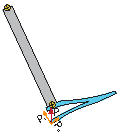
\includegraphics[width=.3\textwidth]{figures/impact_decomposition.pdf}
  \caption{Impact force decomposed}
  \label{fig:impact_decomposition}
\end{figure}

\subsubsection{Profile study} % (fold)
\label{ssub:profile_study}
  The bending effort causes two types of problems: (1) the possible break in the supporting point and (2) the deformation suffered by the beam.
  The break might occur when the internal tensions created are over the ultimate effort in compression or tension of the selected material.
  This is modeled in equation \ref{eq:tension} for symmetric sections and when a single torque $M$ is being applied.
  \begin{equation}
  \label{eq:tension}
    \sigma _{compression} = \sigma _{tension} = \frac{M h_{CG}}{I_x}
  \end{equation}

  Meanwhile the deformation in the extreme can be calculated with the equation \ref{eq:deformation} if the case is simplified to the one depicted in the Figure \ref{fig:bending_case}.
  This is, when the leg is completely stretched to its limits, which is when it will be subjected to the biggest stresses.
  Thus, the leg can be analyzed as a simple straight beam attached to a fixed point with no degrees of freedom, to which a force $P$ (corresponding to $P_{b}$ in \ref{fig:impact_decomposition}) is being applied.

  \begin{figure}[ht!]
    \centering
    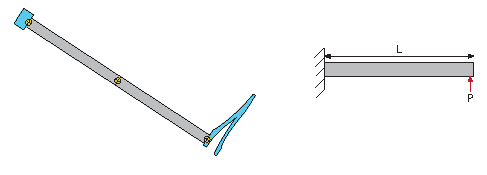
\includegraphics[width=\textwidth]{figures/bending_case.pdf}
    \caption{Simplified representation of the bending case}
    \label{fig:bending_case}
  \end{figure}

  \begin{equation}
  \label{eq:deformation}
    y_L = \frac{P z^2}{6EI}(3L-z) = \frac{P L^2}{6EI}(2L) = \frac{P L^2}{3EI}
  \end{equation}


  For the selected profiles the equations that define the compression ($\sigma _{compression}$) and tension ($\sigma _{tension}$) efforts, along with the deformation in the direction of the applied force ($y_L$) are shown in the table \ref{tab:section_study}, being:

  \begin{enumerate}
    \item $h_{CG}$: height of the center of gravity of the semi-half section from the geometrical center of the section.
    \item $E$: Elastic module.
  \end{enumerate}

  \begin{table}[ht!]
  \centering
  \caption{Stress and deformation analysis for the sections given}
  \label{tab:section_study}
  \begin{tabular}{c|c|c|c|c}
    \textbf{Section} & \textbf{$I$} & \textbf{$h_{CG}$} & \textbf{$y_L$} & \textbf{$\sigma$} \\ \hline
    \raisebox{-.5\height}{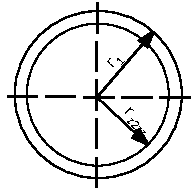
\includegraphics[width=0.25\linewidth]{figures/profile_cylinder.pdf}} & $\frac{\pi}{4} (r_2 ^4 - r_1 ^4)$ & $r_2$ & $\frac{4 P L^2}{3 E \pi(r_2 ^4 - r_1 ^4)}$ & ${\pi(r_2 ^4 - r_1 ^4)} M$ \\ \hline

    \raisebox{-.5\height}{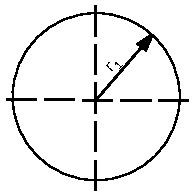
\includegraphics[width=0.25\linewidth]{figures/profile_tube.pdf}} & $\frac{\pi r_1 ^4}{4}$ & $r_1$ & $\frac{4 P L^2}{3 E \pi r_1 ^4}$ & $\frac{4}{\pi r_1 ^3} M$ \\ \hline

    \raisebox{-.5\height}{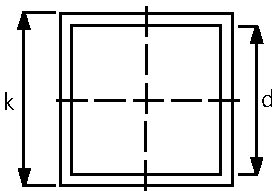
\includegraphics[width=0.33\linewidth]{figures/profile_squared.pdf}} & $\frac{1}{12} (d^4 - k^4)$ & $\frac{d}{2}$ & $\frac{4 P L^2}{E (d^4 - k^4)}$ & $\frac{6 d}{(d^4 - k^4)}$ \\ \hline
  \end{tabular}
  \end{table}
% subsubsection profile_study (end)

\subsubsection{Torque calculation} % (fold)
\label{ssub:torque_calculation}
  For both the profile of the lower and the upper limbs, the torque generated by the impact force determined in the section \ref{sub:impact_force}, is calculated through equation \ref{eq:internal_torque}.
  The torque differs in the limbs due to the fact that the applied on the upper limb is computed with the distance from the foot to the hip while the other one is only from the foot to the knee:
  \begin{equation}
  \begin{aligned}
  \label{eq:internal_torque}
     M_{lower\ limb} = F \cdot l_{link(s)\ length}
  \end{aligned}
  \end{equation}
% subsubsection torque_calculation (end)

\subsubsection{Final limb parameters} % (fold)
\label{ssub:final_limb_parameters}
Using the criteria defined in sections \ref{sec:dimensions} and \ref{sec:physical_properties} for sizes and materials, the presented formulas have been applied to all the profiles of the offered by the provider.
The outputs of the iterative analyses in \ref{cha:design} and \ref{cha:mathematical_model} are shown in the table \ref{tab:limb_physical_properties}. 
This final data is the used for the current stress study.

The profiles have been analyzed calculating the torque from \ref{ssub:torque_calculation} and then applying the section \ref{ssub:profile_study} for each iteration.
The calculations of the last iteration are shown in the appendix \ref{app:profile_selection}.
These results have been then approved or discarded based on a \textit{maximum deformation} and \textit{ultimate tension} requirements, and are shown in the table \ref{tab:profile_selection}

\begin{table}[ht!]
\centering
\caption{Profile selection for each limb}
\label{tab:profile_selection}
\begin{tabular}{c|c|c}
  \textbf{Limb} & \textbf{Section} & \textbf{Dimensions} \\ \hline
  Lower limb & Tube & 20 mm and 1 mm thickness \\ \hline
  Upper limb & Tube & 20 mm and 1 mm thickness 
\end{tabular}
\end{table}

% subsubsection profile_selection (end)



% subsection limb_profile (end) 